\documentclass{article}
\usepackage[UTF8]{ctex}
\usepackage{amsmath}
\usepackage{amsfonts}
\usepackage{mathtools}
\usepackage{jadamath}
% \usepackage{hyperref}
\usepackage[colorlinks=true,linkcolor=blue]{hyperref}
\usepackage{esint}
\usepackage{bm}
\usepackage{braket}
\usepackage{graphicx}
\usepackage{xcolor}
\usepackage{fancyhdr}
\usepackage{geometry}
\usepackage{float}
\usepackage{color}
\usepackage{enumitem}
\usepackage{ulem}
\usepackage{physics}
\usepackage{extarrows}
\usepackage{hyperref}
\usepackage[Symbol]{upgreek}
\usepackage[adjust]{cite}
%opening
\newcommand{\pic}[1]{\begin{wrapfigure}{l}[30cm]{0pt}%
		\includegraphics[width=40mm]{#1}%
\newcommand{\one}{1}
\end{wrapfigure}}
\newgeometry{top=25mm,bottom=25mm,left=25mm,right=40mm}
\title{QM solutions}
\author{}
\date{\today}
\begin{document}

因时间关系以下解释还是找的定性半定量的为主。时间有限,请大家先看下会写简答就好。有关第二个问题大家给出了“原子核壳结构”和“超精细结构”两种答案。事实上老师的意思应该是前者,不过我们都在这里写一下吧。

\begin{enumerate}[label=\textbf{6.\Roman*}, listparindent=\parindent]

\item \emph{Hund定则的半定量解释}


Hund定则是在\textbf{$LS$耦合}方案下解释原子中电子\textbf{基态}排布的规则。(主要参考\href{https://en.wikipedia.org/wiki/Hund\%27s_rules}{维基}上的内容。)

两个关键点:(i) 使用$LS$耦合的原因是当电子序数小于$\sim$40时自旋--轨道耦合项$\xi\vec{L\cdot S}$很弱,多电子哈密顿量(显然是$(H,\vec{J},m_J)$共同本征态)在$(\vec{L}^2,\vec{S}^2)$表象下是近似对角化的,此时$L,\,S$是较好的量子数。当原子序数更大时电子组态会更接近于$(H,\vec{J}_1^2,\vec{J}_2^2)$的共同本征态,需采用$jj$耦合方案分析,Hund定则不再适用。(ii) Hund定则是定性半定量的理论,只适合解释基态电子排布,不能用来分析各组态排序,否则会出bug。

\begin{enumerate}
    \item \emph{定则1:对于给定的电子组态,重数$2S+1$最大的能量最低。}
    
    \emph{举例:$\mathrm{Si}$有两个价电子在$\mathrm{3p^2}$,其轨道角动量都为$l=1$,自旋$s=\frac{1}{2}$。$LS$耦合下总轨道角动量$L=0,1,2$,总自旋$S=0,1$,按照Hund定则基态应当有$S=1$。由于$S=1$自旋波函数是对称的,Pauli不相容原理要求总波函数反对称,则必须空间波函数交换反对称,只能取$L=1$。得到基态的光谱项是三重态$\mathrm{^3P}$。}
    
    解释:首先,自旋$S$最大说明自旋波函数是交换对称的,那么空间波函数则是交换反称的,因此电子不倾向于占据相同轨道。对这一现象存在两种物理解释:一种是说电子占据不同的轨道则离得更远,即$|r_i-r_j|$更大,从而排斥力更小使得整体的能量变低;第二种说,理论计算表明电子不占据同一轨道时整体对原子核的屏蔽效应更弱,相当于与原子核的吸引作用更强,使得能量下降。
    
    \item \emph{定则2:若1中的总自旋量子数相同而不能分辨出基态,则总轨道角动量$L$最大的能量最低。}
    
    \emph{举例:要用到定则2才能解释基态构型的最小的原子是$\mathrm{Ti}$,它有两个价电子在$\mathrm{3d^2}$轨道,其轨道角动量都为$l=2$,自旋$S=\frac{1}{2}$。$LS$耦合下总轨道角动量$L=0,1,2,3,4$,总自旋$S=0,1$。由定则1知道基态构型对应$S=1$,自旋波函数交换对称,因此空间波函数交换反称,此时有$L=1,3$两种情况,即分别对应三重态$\mathrm{^3P_{0,1,2}}$和$\mathrm{^3F_{2,3,4}}$。根据定则2,可知后者的能量更低。}
    
    解释:可以给一个定性解释。对于给定各电子轨道角动量$l_i$,总轨道角动量$L$越大的耦合模式,电子越趋向于同向转动,这样它们相互遇到从而产生排斥的几率小。较少的电子之间的排斥作用意味着整体能量的下降。
    
    \item \emph{定则3:$S$和$L$均相等时,因自旋--轨道耦合会产生进一步能级分裂,需分两种情形:如果电子数不足或等于满壳曾电子数的一半,则总量子数$J$最小的光谱支项能量最低,称为正常次序;反之则$J$最大的能量最低,称为倒转次序。}
    
    \emph{举例:如1中$\mathrm{Si}$的例子,基态的谱项是三重态$\mathrm{^3P_{0,1,2}}$,2个价电子未达到满壳电子数6的一半,因此$J=0$也即光谱支项$\mathrm{^3P_{0}}$是能量最低的。}
    
    解释:对相同的谱项,需要考虑很弱的自旋--轨道耦合作用进一步将多重态的能级劈裂。劈裂项为
    \[\Delta E = \xi \vec{L\cdot S} = \xi(J(J+1)-L(L+1)-S(S+1))\]
    理论给出价电子未达满壳一半时,$\xi$为正,反之为负,因此前者情况下$J$越小能级越低;后者反之。但请注意,不可直接用上面等式解释定则1、2,虽然看上去它对$L$, $S$的要求和定则1、2给出的一致,但它反映的是比1、2引起能级劈裂要更加弱的自旋--轨道耦合作用,只有在1、2都区分不出能级的情况下才会显示出效果。
    
\end{enumerate}

\item \emph{原子核的壳结构}

原子核的壳结构是为了解释质子和中子数取特定值的某些原子核非常稳定的原因。它是用Woods--Saxon势与原子核自身的强自旋--轨道耦合共同解释的。简要地说,这一唯象模型将原子核中多体的强相互作用简化成单粒子在平均势场中的运动,这一势场用介于无限球方势阱和三维谐振子势之间的Woods--Saxon势描述:
\[V(r)==\frac{V_0}{1+\exp[(r-R)/a]}\]
经过数值计算可以得到能级分布规律,但这与实际观测的“幻数”不一致。为解决这一矛盾需引入原子核自身的强自旋--轨道耦合作用
\[\Delta H = \xi(r) \vec{S}\cdot \vec{L}\]
它使得原$(\vec{L}^2,\,\vec{S}^2)$共同本征态下的能级出现很强的劈裂,使得能级分布呈现新的规律(曾书图9.12),与实验观测幻数的排布一致。更细致的说明请参阅曾书9.6节。

\item \emph{原子核的超精细结构}

原子核的超精细结构是原子核的自旋与电子的自旋、轨道角动量耦合,给电子的能级带来的更加细微的劈裂。经典意义上讲,精细结构(电子因自身自旋--轨道耦合引起的能级劈裂)可理解为电子因自旋具有磁矩,在轨道角动量引起的磁场中会产生额外的能量。而超精细结构可理解为原子核因自旋所具有的磁矩在电子的自旋、轨道角动量共同产生的磁场中给整个体系附加的能量。这一附加哈密顿量可化简为:
\[\Delta H =A\vec{I\cdot J}=\frac{1}{2}A\qty(F(F+1)-I(I+1)-J(J+1))\]
(详细的推导在\href{https://en.wikipedia.org/wiki/Hyperfine_structure}{这篇维基}里有,可以先参考\href{https://en.wikipedia.org/wiki/Spin\%E2\%80\%93orbit_interaction}{自旋--轨道耦合的推导})
其中$I$是核自旋,$J$是电子总角动量,$F$是二者总的角动量。它与自旋--轨道耦合的能量项$\xi\vec{L\cdot S}$形式一样,故超精细结构的能级劈裂也满足朗德间隔定则:即劈裂的相邻能级的间隔与总耦合角动量中较大的值成正比。

此外,许多核还有电四级矩,它会与电子在核处产生的电场梯度发生相互作用引起能量的微小改变。这也是超精细结构的原因之一,但它会使能级劈裂偏离朗德间隔定则。

\item \emph{自旋Hall效应的解释}

\emph{自旋霍尔效应是一种运输现象,指载有电流的材料会在两侧形成不同方向自旋的累积,下图展示了方形材料与圆柱形材料中自旋积累的形式。需要注意自选霍尔效应不需要有外加磁场即可实现。}
\begin{figure}[!ht]
    \centering
    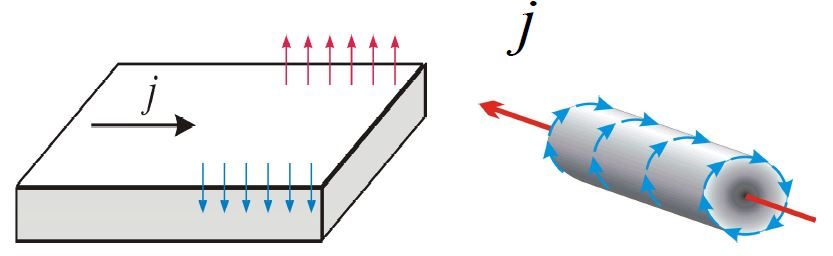
\includegraphics[width=0.5\textwidth]{pic/spin-hall}
\end{figure}

历史上有两个解释(来自\href{https://en.wikipedia.org/wiki/Spin_Hall_effect}{维基})。其一是说流动的电子会与材料中的杂质碰撞发生散射。根据自旋方向的不同,散射的方位角分布也会显示出差异,从而带有不同方向自旋的电子会逐渐弥散到相对的两侧。

第二种解释称这是材料的内禀属性,与杂质无关,它是由电子自旋--轨道相互作用引起的。在不对称的有效电场下因电子的自旋会产生额外的能量项,使得自旋不同的电子有不同的运动轨迹。这和经典力学的马格努斯效应(旋转的乒乓球在空气中轨迹发生偏转)有相似之处。

\end{enumerate}

\end{document}
